\documentclass[10pt]{book}

\usepackage{cdtUsecases}
\usepackage{txfonts}
\title{Entregable C2-EP2\bigskip\\Nombre del Proyecto}
\subtitle{Componente 2 Iteración 2 Especificación del proyecto}
\author{Nombre del equipo o consultoría}
\organization{Escuela Superior de Cómputo, IPN}
\showInstrucciones
\date{\color{red}Borrador del 21 de febrero del 2017\\(para revisión)}
%\date{\color{green}Version 1.0}

%%%%%%%%%%%%%%%%%%%%%%%%%%%%%%%%%%%%%%%%%%%%%%%%%%%%%%%%%%%%%%%%
\begin{document}

\ThisLRCornerWallPaper{1}{theme/bannerAzul}
\maketitle
\thispagestyle{empty}


\frontmatter
\tableofcontents
\listoffigures
\listoftables

\include{projectCharter}

\mainmatter
\LRCornerWallPaper{1}{theme/plecaAyD}

%%%%%%%%%%%%%%%%%%%%%%%%%%%%%%%%%%%%%%%%%%%%%%%%%%%%%%%%%%%%%%%%
\include{3AnalisisDelProblema}
\chapter{Plan de trabajo}	
\label{cap:plantrabajo}

	En este capitulo se especifica el plan de trabajo empelado para el proyecto


\section{Metodología de Trabajo}

\subsection{Marco Metodológico: Scrum Adaptado}
El proyecto se desarrolla bajo un enfoque ágil basado en Scrum, adaptado a las necesidades del equipo y las características del proyecto académico.

\subsubsection{Sprints}
\begin{itemize}
    \item \textbf{Duración:} 2 semanas por sprint
    \item \textbf{Total de sprints:} 6 sprints
    \item \textbf{Duración total:} 12 semanas
\end{itemize}

\subsubsection{Ceremonias Scrum}
\begin{longtable}{|p{3cm}|p{3cm}|p{7cm}|}
\hline
\textbf{Ceremonia} & \textbf{Frecuencia} & \textbf{Descripción} \\
\hline
\endfirsthead

\multicolumn{3}{c}%
{\tablename\ \thetable\ -- \textit{Continuación de la página anterior}} \\
\hline
\textbf{Ceremonia} & \textbf{Frecuencia} & \textbf{Descripción} \\
\hline
\endhead

\hline \multicolumn{3}{r}{\textit{Continúa en la siguiente página}} \\
\endfoot

\hline
\endlastfoot

Sprint Planning & Inicio de cada sprint & Planificación de tareas, definición de objetivos y asignación de historias de usuario \\
\hline
Daily Standup & Lunes, Miércoles, Viernes & Sincronización rápida (15 min) sobre progreso, obstáculos y planes \\
\hline
Sprint Review & Final de cada sprint & Demostración de funcionalidades completadas a stakeholders \\
\hline
Sprint Retrospective & Final de cada sprint & Análisis de mejoras y lecciones aprendidas \\
\hline
\end{longtable}

\subsection{Control de Versiones}
\begin{itemize}
    \item \textbf{Sistema:} Git con GitHub
    \item \textbf{Estrategia de branching:} Git Flow
    \item \textbf{Ramas principales:}
    \begin{itemize}
        \item \texttt{main}: Código en producción
        \item \texttt{develop}: Código en desarrollo
        \item \texttt{feature/*}: Nuevas funcionalidades
        \item \texttt{hotfix/*}: Correcciones urgentes
    \end{itemize}
    \item \textbf{Code Review:} Pull Requests obligatorios con al menos 1 aprobación
\end{itemize}

\subsection{Estándares de Desarrollo}
\begin{itemize}
    \item Código en inglés (variables, funciones, comentarios)
    \item Documentación en español
    \item TypeScript strict mode habilitado
    \item Convenciones de nombres: camelCase para variables, PascalCase para componentes
    \item Commits siguiendo Conventional Commits
\end{itemize}

\section{Organización del Equipo}

\subsection{Roles y Responsabilidades}

\begin{longtable}{|p{3cm}|p{4cm}|p{6cm}|}
\hline
\textbf{Rol} & \textbf{Miembro(s)} & \textbf{Responsabilidades} \\
\hline
\endfirsthead

\multicolumn{3}{c}%
{\tablename\ \thetable\ -- \textit{Continuación de la página anterior}} \\
\hline
\textbf{Rol} & \textbf{Miembro(s)} & \textbf{Responsabilidades} \\
\hline
\endhead

\hline \multicolumn{3}{r}{\textit{Continúa en la siguiente página}} \\
\endfoot

\hline
\endlastfoot

Product Owner & [Aaron Ugalde Téllez] & Definir requisitos, priorizar backlog, validar entregables, comunicación con stakeholders \\
\hline
Scrum Master & [Beltran Saucedo Axel Alejandro] & Facilitar ceremonias, resolver impedimentos, asegurar seguimiento de Scrum \\
\hline
Backend Lead & [Castillo Aldaba Jared] & Diseño de API, arquitectura del servidor, base de datos, seguridad \\
\hline
Frontend Lead & [Vazquez Villagran Jorge] & Arquitectura del cliente, diseño de componentes, UX/UI, integración con API \\
\hline
Desarrollador Full-Stack & [Ugalde Tellez Aaron] & Implementación de features, testing, documentación técnica \\
\hline
QA/Tester & [Beltran Saucedo Axel Alejandro] & Pruebas funcionales, pruebas de integración, documentación de bugs \\
\hline
DevOps & [Castillo Aldaba Jared] & Configuración de entornos, CI/CD, deployment, monitoreo \\
\hline
\end{longtable}

\subsection{Comunicación del Equipo}
\begin{itemize}
    \item \textbf{Herramienta principal:} Discord/Slack
    \item \textbf{Reuniones presenciales:} 2 veces por semana
    \item \textbf{Documentación:} Notion/Confluence
    \item \textbf{Gestión de tareas:} Jira/Trello
    \item \textbf{Repositorio:} GitHub
\end{itemize}

% ============================================
% CRONOGRAMA DE ACTIVIDADES
% ============================================
\section{Cronograma de Actividades}

\subsection{Sprint 0: Planificación e Infraestructura (Semanas 1-2)}

\begin{longtable}{|p{1.5cm}|p{5cm}|p{6.5cm}|}
\hline
\textbf{Día} & \textbf{Actividad} & \textbf{Entregables} \\
\hline
\endfirsthead

\multicolumn{3}{c}%
{\tablename\ \thetable\ -- \textit{Continuación de la página anterior}} \\
\hline
\textbf{Día} & \textbf{Actividad} & \textbf{Entregables} \\
\hline
\endhead

\hline \multicolumn{3}{r}{\textit{Continúa en la siguiente página}} \\
\endfoot

\hline
\endlastfoot

1-2 & Reunión de kick-off & Documento de objetivos y alcance \\
\hline
3-4 & Análisis de requisitos & Documento de requisitos funcionales y no funcionales \\
\hline
5-7 & Diseño de arquitectura & Diagrama de arquitectura, modelo de datos \\
\hline
8-9 & Configuración de repositorio & Repo configurado con estructura de monorepo \\
\hline
10-12 & Setup de entornos & Entorno de desarrollo local configurado \\
\hline
13-14 & Configuración de base de datos & Schema inicial de PostgreSQL \\
\hline
\end{longtable}

\subsection{Sprint 1: Autenticación y Propietarios (Semanas 3-4)}

\textbf{Objetivo:} Implementar el sistema de autenticación y gestión básica de propietarios.

\begin{itemize}
    \item Sistema de registro de propietarios
    \item Login con JWT
    \item Middleware de autenticación
    \item Panel de propietario básico
    \item Gestión de perfil
\end{itemize}

\textbf{Historias de Usuario:}
\begin{itemize}
    \item Como propietario, quiero registrarme en el sistema
    \item Como propietario, quiero iniciar sesión de forma segura
    \item Como propietario, quiero ver y editar mi perfil
\end{itemize}

\subsection{Sprint 2: Gestión de Mascotas (Semanas 5-6)}

\textbf{Objetivo:} Desarrollar el módulo completo de gestión de mascotas.

\begin{itemize}
    \item CRUD de mascotas
    \item Formulario de registro con catálogos (razas, colores, especies)
    \item Listado de mascotas del propietario
    \item Vista detallada de mascota
    \item Validaciones frontend y backend
\end{itemize}

\textbf{Historias de Usuario:}
\begin{itemize}
    \item Como propietario, quiero registrar una mascota
    \item Como propietario, quiero ver todas mis mascotas
    \item Como propietario, quiero editar los datos de mi mascota
\end{itemize}

\subsection{Sprint 3: Historial Médico (Semanas 7-8)}

\textbf{Objetivo:} Implementar el sistema de historial médico completo.

\begin{itemize}
    \item Módulo de vacunas
    \item Módulo de enfermedades
    \item Módulo de alergias
    \item Módulo de desparasitaciones
    \item Subida y gestión de documentos médicos
    \item Vista consolidada de historial
\end{itemize}

\textbf{Historias de Usuario:}
\begin{itemize}
    \item Como propietario, quiero registrar las vacunas de mi mascota
    \item Como propietario, quiero llevar un registro de enfermedades
    \item Como propietario, quiero subir documentos médicos
\end{itemize}

\subsection{Sprint 4: Sistema de Reservaciones (Semanas 9-10)}

\textbf{Objetivo:} Desarrollar el sistema completo de reservaciones.

\begin{itemize}
    \item Catálogo de habitaciones
    \item Creación de reservaciones
    \item Sistema de disponibilidad
    \item Asignación de mascotas a habitaciones
    \item Estados de reservación (pendiente, confirmada, completada)
    \item Cancelación de reservaciones
\end{itemize}

\textbf{Historias de Usuario:}
\begin{itemize}
    \item Como propietario, quiero hacer una reservación para mi mascota
    \item Como propietario, quiero ver mis reservaciones activas
    \item Como admin, quiero confirmar reservaciones
\end{itemize}

\subsection{Sprint 5: Panel Administrativo y Servicios (Semanas 11-12)}

\textbf{Objetivo:} Implementar funcionalidades administrativas y servicios adicionales.

\begin{itemize}
    \item Dashboard administrativo
    \item Gestión de empleados
    \item Catálogo de servicios
    \item Sistema de citas para servicios
    \item Módulo de pagos
    \item Reportes básicos
\end{itemize}

\textbf{Historias de Usuario:}
\begin{itemize}
    \item Como admin, quiero ver todas las reservaciones del hotel
    \item Como admin, quiero gestionar servicios adicionales
    \item Como admin, quiero registrar pagos
\end{itemize}

\subsection{Sprint 6: Testing, Optimización y Deployment (Semanas 13-14)}

\textbf{Objetivo:} Asegurar la calidad del sistema y prepararlo para producción.

\begin{itemize}
    \item Testing exhaustivo de todas las funcionalidades
    \item Corrección de bugs identificados
    \item Optimización de performance (queries, carga de imágenes)
    \item Documentación técnica completa
    \item Documentación de usuario
    \item Deployment a producción
    \item Capacitación al cliente
\end{itemize}

\subsection{Diagrama de Gantt}

\begin{center}
\small
\begin{longtable}{|p{3.5cm}|c|c|c|c|c|c|c|c|c|c|c|c|c|c|}
\hline
\textbf{Actividad} & \multicolumn{14}{c|}{\textbf{Semanas}} \\
\cline{2-15}
& 1 & 2 & 3 & 4 & 5 & 6 & 7 & 8 & 9 & 10 & 11 & 12 & 13 & 14 \\
\hline
\endfirsthead

\multicolumn{15}{c}%
{\tablename\ \thetable\ -- \textit{Continuación de la página anterior}} \\
\hline
\textbf{Actividad} & \multicolumn{14}{c|}{\textbf{Semanas}} \\
\cline{2-15}
& 1 & 2 & 3 & 4 & 5 & 6 & 7 & 8 & 9 & 10 & 11 & 12 & 13 & 14 \\
\hline
\endhead

\hline \multicolumn{15}{r}{\textit{Continúa en la siguiente página}} \\
\endfoot

\hline
\endlastfoot

Sprint 0 & X & X & & & & & & & & & & & & \\
\hline
Sprint 1 & & & X & X & & & & & & & & & & \\
\hline
Sprint 2 & & & & & X & X & & & & & & & & \\
\hline
Sprint 3 & & & & & & & X & X & & & & & & \\
\hline
Sprint 4 & & & & & & & & & X & X & & & & \\
\hline
Sprint 5 & & & & & & & & & & & X & X & & \\
\hline
Sprint 6 & & & & & & & & & & & & & X & X \\
\hline
\end{longtable}
\end{center}

%=========================================================
\chapter{Requerimientos de usuario}
\label{cap:reqUsr}

    En este capitulo se presentan los requerimientos de usuario


%---------------------------------------------------------
\section{Requerimientos de usuario}

\begin{longtable}{|l|p{3cm}|p{7cm}|c|c|}
\caption{Requerimientos funcionales del sistema de gestión de hotel de perros.}
\label{tbl:reqFunc}\\
\hline
ID & Nombre & Descripción & Prioridad & Estado \\
\hline
\endfirsthead

\hline
ID & Nombre & Descripción & Prioridad & Estado \\
\hline
\endhead

\hline
\multicolumn{5}{r}{\footnotesize Continúa en la siguiente página} \\
\endfoot

\hline
\endlastfoot

		\FRitem{RU1}{Gestión de Empleados}{El usuario requiere llevar un registro actualizado de todos los empleados del hotel, incluyendo sus datos personales, información laboral (puesto, salario, fecha de contratación), datos de contacto y estado (activo/inactivo). El sistema debe permitir crear, modificar, consultar y dar de baja empleados.}{1}{\DONE}
		
		\FRitem{RU2}{Gestión de Propietarios}{El usuario requiere llevar un registro completo de los propietarios de mascotas, incluyendo datos personales, múltiples teléfonos de contacto, direcciones y su historial de reservaciones. El sistema debe facilitar la búsqueda rápida y actualización de información de contacto.}{1}{\DONE}
		
		\FRitem{RU3}{Gestión de Mascotas}{El usuario requiere mantener un registro detallado de cada mascota hospedada, incluyendo datos de identificación (nombre, especie, raza, color, sexo, fecha de nacimiento), historial médico completo (vacunaciones, desparasitaciones, enfermedades, alergias), documentos asociados y fotografías.}{1}{\DONE}
		
		\FRitem{RU4}{Sistema de Reservaciones}{El usuario requiere gestionar las reservaciones de hospedaje con un calendario visual interactivo que muestre la disponibilidad de habitaciones, permita crear nuevas reservas, asignar habitaciones, controlar check-in/check-out y llevar el seguimiento del estado de cada reservación.}{1}{\DONE}
		
		\FRitem{RU5}{Control de Habitaciones}{El usuario requiere llevar un registro actualizado de todas las habitaciones disponibles en el hotel, su capacidad, tipo, características especiales, estado de mantenimiento y disponibilidad para reservaciones.}{1}{\DONE}
		
		\FRitem{RU6}{Gestión de Servicios Adicionales}{El usuario requiere ofrecer y gestionar servicios complementarios al hospedaje tales como atención veterinaria, peluquería canina, entrenamiento y otros servicios especializados, con control de horarios, empleados asignados y tarifas.}{2}{\DONE}
		
		\FRitem{RU7}{Programación de Citas}{El usuario requiere un sistema de agendamiento para servicios especializados que permita programar citas, asignar empleados calificados, evitar conflictos de horario y llevar seguimiento del estado de cada cita (pendiente, realizada, cancelada).}{2}{\DONE}
		
		\FRitem{RU8}{Registro de Vacunaciones}{El usuario requiere mantener un historial completo y actualizado de todas las vacunas aplicadas a cada mascota, incluyendo tipo de vacuna, fecha de aplicación, fecha de próxima dosis y observaciones del veterinario.}{1}{\DONE}
		
		\FRitem{RU9}{Gestión de Documentos}{El usuario requiere almacenar, visualizar y gestionar documentos digitales importantes de cada mascota como certificados veterinarios, cartillas de vacunación, resultados de análisis y otros documentos oficiales en formatos PDF e imagen.}{2}{\DONE}
		
		\FRitem{RU10}{Control de Pagos}{El usuario requiere llevar un registro detallado de todos los pagos realizados por los clientes, métodos de pago utilizados, montos, fechas y asociarlos con las reservaciones o servicios correspondientes para control financiero.}{1}{\TODO}
		
		\FRitem{RU11}{Sistema de Autenticación}{El usuario requiere un sistema seguro de inicio de sesión que identifique a cada empleado y controle el acceso a las diferentes funcionalidades del sistema según su rol.}{1}{\DONE}
		
		\FRitem{RU12}{Control de Acceso por Roles}{El usuario requiere que el sistema restrinja las operaciones que cada empleado puede realizar según su puesto.}{1}{\DONE}
		
		\FRitem{RU13}{Historial de Hospedajes}{El usuario requiere consultar el historial completo de hospedajes de cada mascota para conocer fechas anteriores, habitaciones utilizadas, servicios contratados y cualquier incidente o nota relevante registrada.}{2}{\TODO}
		
		\FRitem{RU14}{Asignación de Empleados a Servicios}{El usuario requiere asignar empleados específicos a cada cita o servicio programado, considerando su especialización y disponibilidad, para garantizar la calidad del servicio.}{2}{\DONE}
		
		\FRitem{RU15}{Búsqueda y Filtros Avanzados}{El usuario requiere herramientas de búsqueda rápida y filtros para localizar fácilmente mascotas, propietarios, empleados y reservaciones usando criterios múltiples como nombre, fecha o estado.}{2}{\TODO}
		
		\FRitem{RU16}{Notificaciones de Vencimientos}{El usuario requiere recibir alertas automáticas sobre vacunas próximas a vencer, reservaciones próximas, pagos pendientes y otras fechas importantes.}{3}{\TODO}
		
		\FRitem{RU17}{Reportes de Ocupación}{El usuario requiere generar reportes periódicos sobre la ocupación del hotel, ingresos por período, servicios más solicitados y otros indicadores clave.}{3}{\TODO}
		
		\FRitem{RU18}{Gestión de Fotografías}{El usuario requiere almacenar y visualizar múltiples fotografías de cada mascota para su identificación visual y seguimiento durante el hospedaje.}{2}{\DONE}
		
		\FRitem{RU19}{Registro de Observaciones}{El usuario requiere documentar observaciones diarias sobre el comportamiento, alimentación, salud y cualquier incidente relevante de cada mascota durante su estancia.}{2}{\TODO}
		
		\FRitem{RU20}{Calendario Interactivo}{El usuario requiere una vista de calendario visual e interactiva que muestre todas las reservaciones, disponibilidad de habitaciones y citas de servicios.}{1}{\DONE}
		
		\FRitem{RU21}{Validación de Datos}{El usuario requiere que el sistema valide automáticamente la información ingresada para prevenir errores e inconsistencias.}{1}{\DONE}
		
		\FRitem{RU22}{Interfaz Responsiva}{El usuario requiere que el sistema sea accesible desde distintos dispositivos manteniendo funcionalidad y usabilidad.}{2}{\TODO}
		
		\FRitem{RU23}{Copia de Seguridad Automática}{El usuario requiere que el sistema realice respaldos automáticos periódicos de toda la información.}{1}{\TODO}
		
		\FRitem{RU24}{Auditoría de Cambios}{El usuario requiere llevar un registro de las modificaciones importantes realizadas en el sistema.}{3}{\TODO}
		
		\FRitem{RU25}{Exportación de Datos}{El usuario requiere exportar información del sistema en formatos estándar para análisis externo o respaldo.}{3}{\TODO}
        
        \FRitem{RU26}{Manejo de Habitaciones}{El usuario requiere administrar de forma detallada las habitaciones del hotel, incluyendo su alta, modificación y baja, así como la gestión de su capacidad, tipo, características especiales, estado de mantenimiento y disponibilidad para reservaciones.}{1}{\TODO}

        \FRitem{RU27}{Perfil de Empleado}{El usuario requiere que cada empleado cuente con un perfil individual que muestre su información personal, puesto, rol asignado, horarios, servicios que puede realizar y su historial de actividades dentro del sistema.}{2}{\TODO}

        \FRitem{RU28}{Manejo de Catálogos}{El usuario requiere gestionar los catálogos del sistema, tales como razas, tipos de servicios, tipos de habitaciones, estados, roles y otros datos parametrizables, permitiendo su creación, modificación y eliminación para mantener la flexibilidad del sistema.}{2}{\TODO}

		
	\end{longtable}

{\footnotesize\em Para leer correctamente esta tabla vea la leyenda en la Tabla~\ref{tbl:leyendaRF}.}



%=========================================================
\section{Requerimientos No Funcionales}
\label{sec:reqNoFunc}

En esta sección se presentan los requerimientos no funcionales del sistema, que especifican propiedades de calidad, restricciones y atributos que el sistema debe cumplir para garantizar su correcto funcionamiento, seguridad, rendimiento y mantenibilidad.

\begin{NFRequerimientos}
	\NFRitem{RNF1}{Seguridad}{
		El sistema debe garantizar que únicamente usuarios autenticados y autorizados puedan acceder a las funcionalidades del sistema mediante mecanismos robustos de autenticación y control de acceso basado en roles.
	}{
		Implementar autenticación mediante contraseñas encriptadas con bcrypt, control de acceso basado en roles (RBAC), sesiones con tokens JWT que expiren tras 7 días de inactividad, validación de permisos en cada operación sensible, y uso de HTTPS para comunicaciones.
	}{Crítica}
	
	\NFRitem{RNF2}{Rendimiento}{
		El sistema debe responder de forma ágil y eficiente ante las solicitudes del usuario, ejecutando operaciones en tiempos aceptables para no afectar la experiencia de usuario.
	}{
		Optimizar consultas a base de datos mediante índices apropiados, implementar caché para datos frecuentemente consultados, minimizar procesamiento innecesario en el cliente, establecer timeouts adecuados. Tiempo objetivo: consultas $<$ 1 segundo, operaciones de registro $<$ 2 segundos.
	}{Alta}
	
	\NFRitem{RNF3}{Escalabilidad}{
		El sistema debe permitir el crecimiento en volumen de datos y número de usuarios sin afectar su estabilidad ni requerir rediseños arquitectónicos mayores. Debe estar diseñado de forma modular y desacoplada.
	}{
		Utilizar arquitectura en capas claramente separadas (presentación, lógica de negocio, acceso a datos), aplicar principios SOLID para facilitar extensión, diseñar módulos independientes con interfaces bien definidas, implementar API RESTful stateless para permitir escalamiento horizontal.
	}{Alta}
	
	\NFRitem{RNF4}{Usabilidad}{
		El sistema debe proporcionar una interfaz clara, intuitiva y fácil de utilizar donde los usuarios puedan completar sus tareas de manera sencilla, con retroalimentación clara y prevención de errores.
	}{
		Diseñar interfaz consistente en todas las pantallas, implementar validación en tiempo real de formularios, proporcionar mensajes de error claros y específicos en español, usar retroalimentación visual para todas las acciones del usuario (loading states, confirmaciones), aplicar principios de diseño UX modernos.
	}{Alta}
	
	\NFRitem{RNF5}{Disponibilidad}{
		El sistema debe estar disponible y funcionar correctamente durante su horario operativo, manejando fallos de forma controlada y evitando la pérdida de información.
	}{
		Implementar manejo robusto de excepciones en todas las capas, registrar errores en logs para análisis posterior, realizar respaldos automáticos periódicos de datos críticos, diseñar mecanismos de recuperación ante fallos, establecer monitoreo del estado del sistema.
	}{Alta}
	
	\NFRitem{RNF6}{Mantenibilidad}{
		El sistema debe facilitar la comprensión, modificación y evolución del código por parte del equipo de desarrollo mediante código claro, estructurado y siguiendo buenas prácticas de programación.
	}{
		Aplicar convenciones de nomenclatura consistentes (camelCase para variables/métodos, PascalCase para clases/componentes), documentar código y funciones complejas mediante comentarios descriptivos, estructurar el proyecto de forma lógica y modular, seguir estándares de codificación establecidos (ESLint, Prettier), realizar revisiones de código en equipo.
	}{Media}
	
	\NFRitem{RNF7}{Compatibilidad}{
		El sistema debe funcionar correctamente en distintos entornos de ejecución, navegadores web modernos y sistemas operativos, sin requerir configuraciones especiales del usuario final.
	}{
		Utilizar tecnologías web estándar (HTML5, CSS3, JavaScript ES6+), probar funcionamiento en navegadores principales (Chrome, Firefox, Safari, Edge versiones recientes), diseñar para diferentes resoluciones de pantalla (responsive design), facilitar despliegue en diferentes entornos (desarrollo, staging, producción) mediante variables de configuración.
	}{Media}
	
	\NFRitem{RNF8}{Integridad de Datos}{
		El sistema debe garantizar que la información almacenada sea correcta, consistente y coherente, validando los datos antes de ser almacenados y manteniéndolos íntegros durante todo su ciclo de vida.
	}{
		Implementar validación de datos en múltiples capas (cliente y servidor), establecer restricciones de integridad en base de datos (claves foráneas, valores únicos, NOT NULL, CHECK constraints), validar tipos y formatos de datos, implementar transacciones ACID para operaciones críticas, proporcionar mensajes claros de error de validación al usuario.
	}{Crítica}
	
	\NFRitem{RNF9}{Respaldo y Recuperación}{
		El sistema debe contar con mecanismos automatizados de respaldo de información y procedimientos documentados para recuperación ante desastres o pérdida de datos.
	}{
		Implementar respaldos automáticos diarios de la base de datos completa, mantener respaldos incrementales cada 6 horas, almacenar respaldos en ubicación separada del servidor principal, documentar procedimientos de restauración, probar periódicamente la recuperación de respaldos.
	}{Alta}
	
	\NFRitem{RNF10}{Auditabilidad}{
		El sistema debe mantener un registro de las operaciones críticas realizadas, identificando quién realizó cada acción, cuándo y sobre qué datos, para fines de auditoría y rastreo de problemas.
	}{
		Registrar en logs todas las operaciones de creación, modificación y eliminación de datos sensibles, incluir timestamp, usuario responsable y datos modificados en cada registro, implementar sistema de logs centralizado con niveles de severidad (ERROR, WARN, INFO), permitir consulta y filtrado de logs por administradores.
	}{Media}
	
	\NFRitem{RNF11}{Privacidad}{
		El sistema debe proteger la información personal de los usuarios y cumplir con regulaciones de protección de datos aplicables, limitando el acceso a información sensible solo a usuarios autorizados.
	}{
		Encriptar contraseñas usando algoritmos fuertes (bcrypt con salt), no almacenar información de tarjetas de crédito en el sistema, implementar políticas de privacidad claras, permitir a propietarios consultar y modificar únicamente sus propios datos, limitar acceso de empleados a información estrictamente necesaria para su rol.
	}{Crítica}
	
	\NFRitem{RNF12}{Confiabilidad}{
		El sistema debe operar de manera predecible y consistente, minimizando errores, comportamientos inesperados y caídas del sistema durante su operación normal.
	}{
		Implementar pruebas unitarias para componentes críticos, realizar pruebas de integración entre módulos, validar todas las entradas de usuario antes de procesarlas, manejar casos excepcionales de forma explícita (conexiones de red fallidas, datos faltantes), implementar circuit breakers para servicios externos.
	}{Alta}
	
	\NFRitem{RNF13}{Portabilidad}{
		El sistema debe poder ser desplegado en diferentes entornos de hosting y proveedores cloud sin requerir modificaciones significativas en el código fuente.
	}{
		Utilizar contenedores Docker para empaquetar la aplicación con todas sus dependencias, externalizar configuración mediante variables de ambiente (.env), documentar requerimientos de infraestructura (versiones de Node.js, PostgreSQL), evitar dependencias de servicios propietarios de proveedores específicos.
	}{Media}
	
	\NFRitem{RNF14}{Documentación}{
		El sistema debe estar acompañado de documentación técnica completa y actualizada que facilite su instalación, configuración, uso y mantenimiento por parte de desarrolladores y administradores.
	}{
		Mantener archivo README.md con instrucciones de instalación y ejecución, documentar API REST con descripción de endpoints, parámetros y respuestas, incluir ejemplos de uso de funcionalidades principales, documentar modelo de base de datos con diagrama ER y descripción de tablas, mantener changelog con registro de cambios por versión.
	}{Media}
	
	\NFRitem{RNF15}{Internacionalización}{
		El sistema debe estar preparado para soportar múltiples idiomas en el futuro, separando textos de la interfaz de usuario del código de la aplicación.
	}{
		Externalizar todos los textos mostrados al usuario en archivos de configuración separados (archivos de traducción), utilizar biblioteca de i18n (internacionalización) compatible con React, codificar cadenas de texto en UTF-8 para soportar caracteres especiales, diseñar interfaz considerando expansión/contracción de textos en diferentes idiomas.
	}{Baja}
\end{NFRequerimientos}

{\footnotesize\em Los requerimientos no funcionales complementan los funcionales estableciendo propiedades de calidad que el sistema debe cumplir.}

\include{6ModeloDelNegocio}
\include{7ModeloDinamico}
%=========================================================
\chapter{Modelo de la interacción}	
\label{cap:modInteraccion}

En este capítulo se describe el diseño de la interacción del Sistema de Gestión para Hotel de Perros. Se presenta el modelo de navegación que ilustra las relaciones y flujos entre las diferentes pantallas del sistema, así como las especificaciones detalladas de cada interfaz de usuario, incluyendo su propósito, elementos, comportamiento y los mensajes del sistema.

El diseño de la interacción es fundamental para garantizar una experiencia de usuario coherente, intuitiva y eficiente, facilitando el cumplimiento de los objetivos de los usuarios y minimizando la curva de aprendizaje del sistema.

\section{Generalidades del Diseño de Interacción}

El diseño de las interfaces del Sistema de Gestión para Hotel de Perros sigue los siguientes principios fundamentales:

\subsection{Consistencia Visual y Funcional}
Todas las pantallas mantienen una estructura visual coherente mediante el uso de:
\begin{itemize}
    \item \textbf{Sistema de diseño unificado:} Implementado con Tailwind CSS v4, garantizando consistencia en colores, tipografía, espaciados y componentes.
    \item \textbf{Componentes reutilizables:} Botones, formularios, tarjetas y modales siguen patrones consistentes en toda la aplicación.
    \item \textbf{Iconografía semántica:} Uso de la biblioteca Lucide React para iconos claros y comprensibles.
    \item \textbf{Header persistente:} Barra de navegación superior presente en todas las pantallas autenticadas.
\end{itemize}

\subsection{Retroalimentación al Usuario}
El sistema proporciona retroalimentación constante mediante:
\begin{itemize}
    \item \textbf{Estados de carga:} Indicadores visuales durante operaciones asíncronas (spinners, skeleton screens).
    \item \textbf{Mensajes de confirmación:} Notificaciones de éxito tras completar acciones importantes.
    \item \textbf{Mensajes de error descriptivos:} Explicaciones claras sobre problemas y cómo resolverlos.
    \item \textbf{Validación en tiempo real:} Feedback inmediato en formularios sobre errores de formato o campos faltantes.
    \item \textbf{Efectos hover:} Cambios visuales al posicionar el cursor sobre elementos interactivos.
\end{itemize}


\subsection{Prevención y Manejo de Errores}
El diseño incluye mecanismos para prevenir y manejar errores:
\begin{itemize}
    \item \textbf{Validación preventiva:} Campos de formulario con restricciones de formato y tipo de dato.
    \item \textbf{Confirmaciones para acciones destructivas:} Diálogos de confirmación antes de eliminar registros.
    \item \textbf{Deshabilitación de botones:} Botones inactivos hasta que se cumplan las condiciones necesarias.
    \item \textbf{Mensajes contextuales:} Ayudas y sugerencias cerca de campos que requieren formato específico.
\end{itemize}


\subsection{Diseño Responsive}
Las interfaces se adaptan a diferentes tamaños de pantalla:
\begin{itemize}
    \item \textbf{Mobile-first approach:} Diseño optimizado primero para dispositivos móviles.
    \item \textbf{Breakpoints adaptativos:} Layouts que se reorganizan según el espacio disponible.
    \item \textbf{Navegación contextual:} Menús que se ajustan según el dispositivo (drawer en móvil, sidebar en desktop).
\end{itemize}


\subsection{Accesibilidad}
El sistema considera principios de accesibilidad web (WCAG 2.1):
\begin{itemize}
    \item \textbf{Contraste suficiente:} Texto legible con relación de contraste adecuada.
    \item \textbf{Navegación por teclado:} Todos los elementos interactivos accesibles vía teclado.
    \item \textbf{Etiquetas semánticas:} HTML semántico para lectores de pantalla.
    \item \textbf{Textos alternativos:} Descripciones en imágenes e iconos importantes.
\end{itemize}


\section{Modelo de navegación}

El modelo de navegación representa la estructura de flujos entre las diferentes pantallas del sistema. La Figura~\ref{fig:mapa} muestra el mapa de navegación completo, donde se pueden identificar los siguientes flujos principales:

\begin{figure}[htbp]
	\begin{center}
		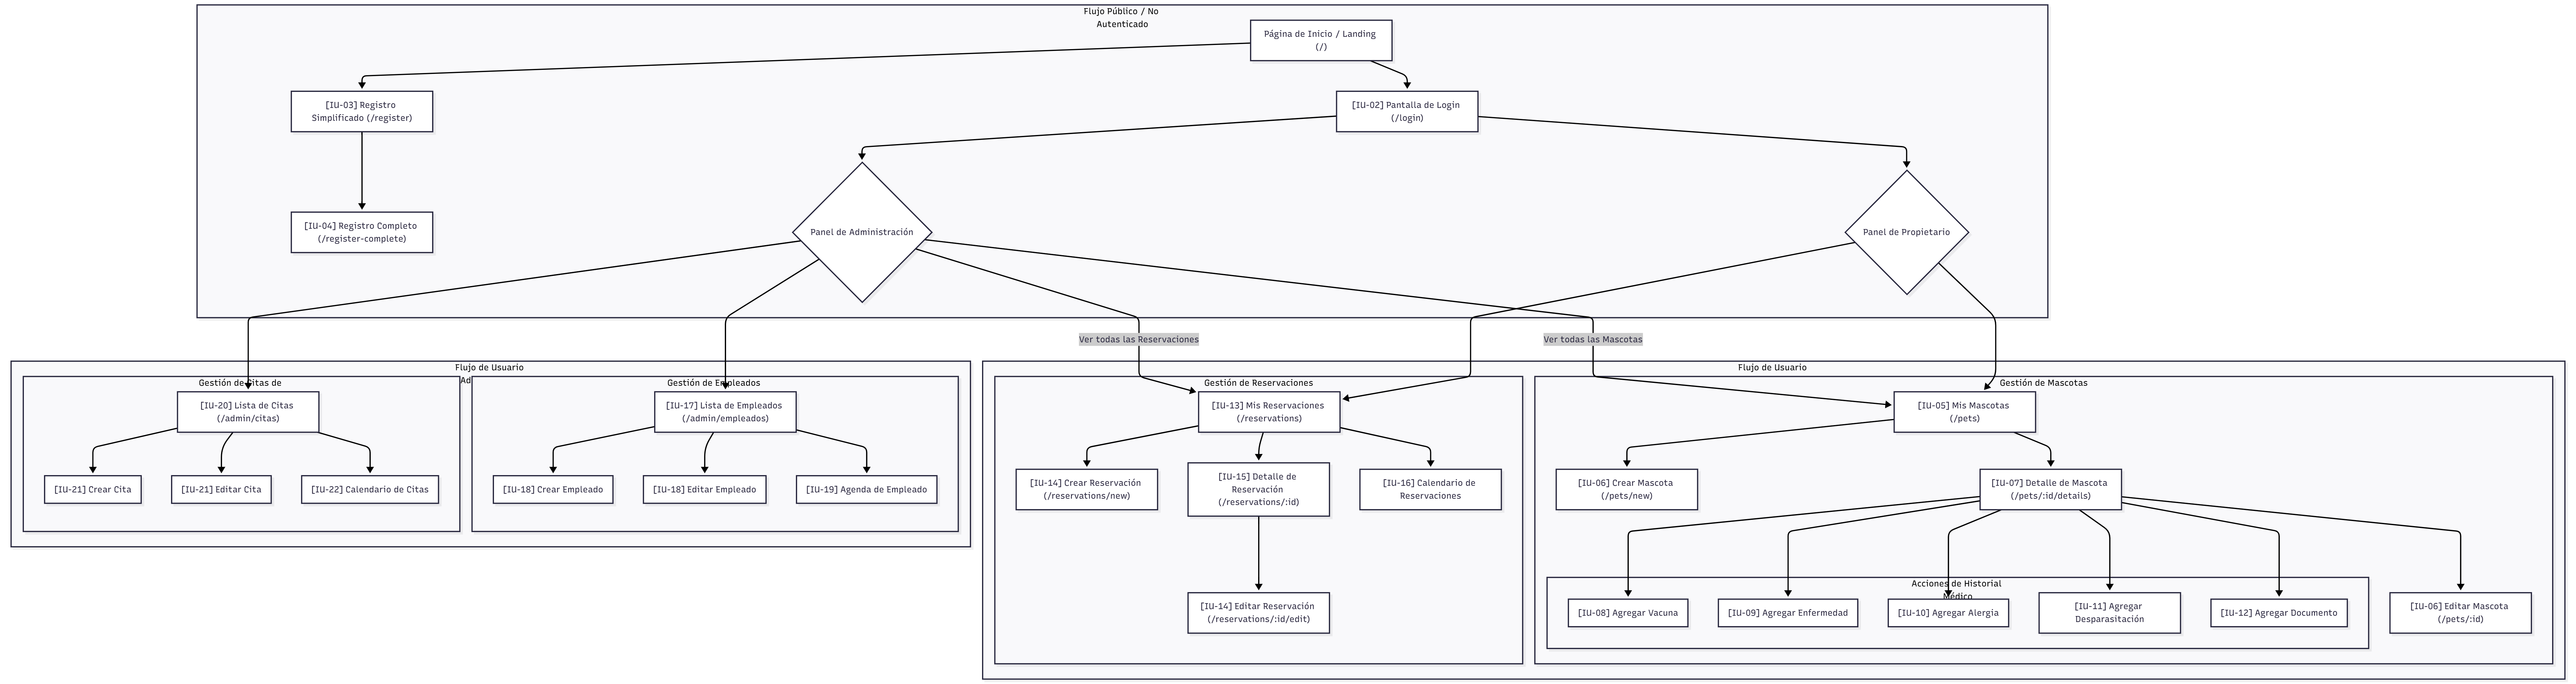
\includegraphics[width=.9\textwidth]{images/mapa}
		\caption{Mapa de Navegación del Sistema}
		\label{fig:mapa}
	\end{center}
\end{figure}



%--------------------------------------
\section{IU-01 Página de Inicio / Landing}

\subsection{Objetivo}
    Servir como punto de entrada y presentación del servicio de Hotel para Perros, informando a los usuarios sobre las funcionalidades principales y guiándolos hacia el registro, inicio de sesión o creación de reservaciones.

\subsection{Diseño}
    Esta pantalla \IUref{IU-01}{Página de Inicio / Landing} (ver figura~\ref{IU-01}) aparece al iniciar la aplicación o al navegar a la ruta raíz `/`. Está diseñada de forma informativa, compuesta por varias secciones visuales como una principal (Hero) con un mensaje de bienvenida y llamada a la acción, una sección de preguntas frecuentes, una de contacto y otra de llamado a la acción. Incluye un encabezado superior (`Header`) persistente con opciones de navegación global.

\IUfig[.5]{IU01}{IU-01}{Página de Inicio / Landing.}

\subsection{Salidas}
    Ninguna.

\subsection{Entradas}
    Ninguna.

\subsection{Comandos}
\begin{itemize}
    \item \IUbutton{Reservar}: Inicia el flujo para crear una nueva reservación. Si el usuario no está autenticado, lo redirige a la \IUref{IU-02}{Pantalla de Login}. Si ya está autenticado, lo lleva al formulario de reservación \IUref{IU-14}{Formulario de Reservación}.
    \item \IUbutton{Más}: Proporciona información adicional sobre el servicio o funcionalidades, posiblemente redirigiendo a una página interna o sección de la misma.
    \item \IUbutton{Contacto}: Redirige al usuario a la sección de contacto dentro de la página o a una pantalla dedicada para resolver dudas.
    \item \IUbutton{Iniciar sesión}: Redirige a la \IUref{IU-02}{Pantalla de Login} para que el usuario acceda a su cuenta. (Disponible en el Header).
    \item \IUbutton{Unirse}: Redirige a la \IUref{IU-03}{Pantalla de Registro Simplificado} para que nuevos usuarios creen una cuenta. (Disponible en el Header).
\end{itemize}

\subsection{Mensajes}
\begin{itemize}
    \item Ninguno. Esta pantalla es principalmente informativa y de navegación, sin validaciones o procesos que generen mensajes de usuario directamente desde este componente principal.
\end{itemize}


%--------------------------------------
\section{IU-02 Pantalla de Login}

\subsection{Objetivo}
    Permitir a los usuarios registrados acceder al sistema mediante la introducción de sus credenciales (correo electrónico y contraseña) para iniciar una sesión autenticada.

\subsection{Diseño}
    Esta pantalla \IUref{IU-02}{Pantalla de Login} (ver figura~\ref{IU-02}) aparece al acceder directamente a la ruta `/login` o al intentar acceder a rutas protegidas sin estar previamente autenticado. Presenta un formulario centrado con campos para el correo electrónico y la contraseña, acompañado de un botón principal para iniciar sesión. Incluye un icono que permite alternar la visibilidad de la contraseña y una imagen decorativa de un perro para realzar la estética.

\IUfig[.5]{IU02}{IU-02}{Pantalla de Login.}

\subsection{Salidas}
    Ninguna.

\subsection{Entradas}
\begin{itemize}
    \item Correo electrónico (campo de texto, tipo email)
    \item Contraseña (campo de texto, tipo password)
\end{itemize}

\subsection{Comandos}
\begin{itemize}
    \item \IUbutton{Iniciar Sesión}: Valida las credenciales ingresadas. Si son correctas, el sistema inicia la sesión del usuario, establece una cookie de autenticación y redirige al usuario a la página de inicio (`/`) o a la última página protegida a la que intentó acceder. Si hay un error, muestra un mensaje relevante.
    \item \IUbutton{Ojo/Ojo Tachado}: Alterna la visibilidad del texto ingresado en el campo de contraseña, permitiendo al usuario verificar lo que escribe.
\end{itemize}

\subsection{Mensajes}
\begin{itemize}
    \item Credenciales inválidas: Se muestra si el correo electrónico o la contraseña no coinciden con un usuario registrado.
    \item Error al iniciar sesión: Mensaje genérico en caso de un fallo inesperado durante el proceso de login.
\end{itemize}

%--------------------------------------
\section{IU-03 Pantalla de Registro de Usuario}

\subsection{Objetivo}
    Permitir a nuevos usuarios crear una cuenta de propietario básica en el sistema, proporcionando su información personal esencial y credenciales de acceso (correo y contraseña).

\subsection{Diseño}
    Esta pantalla \IUref{IU-03}{Pantalla de Registro de Usuario} (ver figura~\ref{IU-03}) aparece cuando un usuario no registrado accede a la ruta `/register`, normalmente a través de un enlace en la página de inicio o de login. Presenta un formulario de registro que solicita datos personales (nombre, apellidos), correo electrónico y una contraseña, la cual debe ser confirmada. Incluye enlaces para navegar hacia la pantalla de inicio de sesión o al formulario de registro completo.

\IUfig[.5]{UI03}{IU-03}{Pantalla de Registro de Usuario.}
\IUfig[.5]{UI03-2}{IU-03}{Pantalla de Registro de Usuario.}
\subsection{Salidas}
    Ninguna.

\subsection{Entradas}
\begin{itemize}
    \item Correo Electrónico
    \item Nombre
    \item Primer Apellido
    \item Segundo Apellido (opcional)
    \item Contraseña
    \item Confirmar Contraseña
\end{itemize}

\subsection{Comandos}
\begin{itemize}
    \item \IUbutton{Crear Cuenta}: Valida que los datos ingresados sean correctos (contraseñas coinciden, campos requeridos llenos). Si la validación es exitosa, envía la información al servidor para crear una nueva cuenta de propietario, inicia la sesión del nuevo usuario y lo redirige a la página de inicio (`/`).
    \item \IUbutton{Iniciar Sesión}: Redirige al usuario a la \IUref{IU-02}{Pantalla de Login}.
    \item \IUbutton{Ir a Registro Completo}: Redirige al usuario al \IUref{IU-04}{Formulario de Registro Completo} para un registro con más detalles.
    \item \IUbutton{Ojo/Ojo Tachado}: Alterna la visibilidad del texto en los campos de contraseña y confirmación de contraseña.
\end{itemize}

\subsection{Mensajes}
\begin{itemize}
    \item Las contraseñas no coinciden: Se muestra si el contenido de los campos "Contraseña" y "Confirmar Contraseña" no es idéntico.
    \item La contraseña debe tener al menos 6 caracteres: Se muestra si la contraseña no cumple con la longitud mínima requerida.
    \item Nombre y primer apellido son requeridos: Se muestra si los campos de nombre o primer apellido están vacíos.
    \item Correo electrónico ya registrado: Se muestra si el servidor rechaza el registro porque el correo ya existe en la base de datos.
    \item Error al registrar usuario: Mensaje genérico en caso de un fallo inesperado del servidor durante el proceso de registro.
\end{itemize}

%--------------------------------------
\section{IU-04 Pantalla de Perfil de Propietario}

    3 \subsection{Objetivo}
    4     Permitir a un nuevo usuario realizar un registro completo y detallado, incluyendo su información personal, múltiples contactos telefónicos y
      direcciones de estancia, para crear un perfil de propietario exhaustivo en una sola operación.

    6 \subsection{Diseño}
    7     Esta pantalla \IUref{IU-04}{Pantalla de Perfil de Propietario} (ver figura~\ref{IU-04}) aparece cuando un usuario navega a la ruta
      `/register-complete`. Aunque el nombre del caso de uso es "perfil de propietario", esta interfaz funciona como un formulario de "Registro Completo".
      Está organizada en tres secciones principales: "Información Personal" para los datos de la cuenta y credenciales, "Teléfonos de Contacto" donde se
      pueden agregar dinámicamente varios números, y "Direcciones Durante el Hospedaje" para registrar las ubicaciones del propietario durante la estancia d
      su mascota.

    9 \IUfig[.5]{IU04}{IU-04}{Pantalla de Perfil de Propietario (Registro Completo).}

   11 \subsection{Salidas}
   12     Ninguna.

   14 \subsection{Entradas}
   15 \begin{itemize}
   16     \item \textbf{Información Personal:} Correo Electrónico, Contraseña, Confirmar Contraseña, Nombre, Apellidos.
   17     \item \textbf{Teléfonos (por cada uno):} Número, Tipo de Teléfono, Nombre de Contacto, Relación, si es Principal, Notas.
   18     \item \textbf{Direcciones (por cada una):} Tipo de Domicilio, Código Postal, Estado, Municipio, Colonia, Calle, Números, Fechas de Estancia, si es
      Predeterminada, Notas.
   19 \end{itemize}

   21 \subsection{Comandos}
   22 \begin{itemize}
   23     \item \IUbutton{Registrarse}: Valida la completitud y corrección de todos los datos ingresados en las tres secciones. Si la validación es exitosa,
      envía toda la información al servidor para crear la cuenta de propietario. En caso de éxito, muestra una alerta y redirige a la pantalla de login.
   24     \item \IUbutton{Cancelar}: Descarta todos los datos ingresados y redirige al usuario a la pantalla de login.
   25     \item \IUbutton{+ Agregar} (en Teléfonos/Direcciones): Añade un nuevo bloque de campos para que el usuario pueda registrar un teléfono o una direc
      ón adicional.
   26     \item \IUbutton{Eliminar} (Icono de bote de basura): Elimina el bloque de teléfono o dirección correspondiente.
   27 \end{itemize}

   29 \subsection{Mensajes}
   30 \begin{itemize}
   31     \item Por favor completa todos los campos obligatorios.
   32     \item Las contraseñas no coinciden.
   33     \item La contraseña debe tener al menos 6 caracteres.
   34     \item Debe agregar al menos un teléfono.
   35     \item ¡Registro exitoso! Ahora puedes iniciar sesión.
   36     \item Error al registrar. Por favor intenta de nuevo.
   37     \item No se encontró información para el código postal ingresado.
   38 \end{itemize}

%--------------------------------------
\section{IU-05 Pantalla de Consulta de Mascotas}

\subsection{Objetivo}
    Proporcionar al Propietario una vista general de todas sus mascotas registradas, y servir como punto de partida para realizar acciones de gestión como agregar, editar, eliminar o consultar el detalle de cada una.

\subsection{Diseño}
    Esta pantalla \IUref{IU-05}{Pantalla de Consulta de Mascotas} (ver figura~\ref{IU-05}) aparece cuando el usuario autenticado navega a la ruta `/pets`. Presenta una cabecera con el título "Mis Mascotas" y un botón principal para agregar un nuevo animal. El contenido principal es una cuadrícula de tarjetas, donde cada tarjeta representa una mascota y muestra su información básica (nombre, especie, etc.). Si no hay mascotas registradas, la pantalla muestra un mensaje indicándolo.

\IUfig[.5]{IU05}{IU-05}{Pantalla de Consulta de Mascotas.}

\subsection{Salidas}
\begin{itemize}
    \item Lista de tarjetas, cada una representando una mascota con su información clave: Nombre, ID, Especie, Sexo, Fecha de Nacimiento y Peso.
    \item Para usuarios administradores, se muestra adicionalmente el Nombre y Correo del Propietario en cada tarjeta.
\end{itemize}

\subsection{Entradas}
    Ninguna.

\subsection{Comandos}
\begin{itemize}
    \item \IUbutton{Agregar Mascota}: Redirige al usuario al \IUref{IU-06}{Formulario de Mascota} para registrar un nuevo animal.
    \item \IUbutton{Tarjeta de Mascota} (al hacer clic en el área principal de la tarjeta): Redirige al usuario a la \IUref{IU-07}{Pantalla de Detalle de Mascota} para ver la información completa del animal seleccionado.
    \item \IUbutton{Editar} (botón en cada tarjeta): Redirige al usuario al \IUref{IU-06}{Formulario de Mascota} en modo de edición, precargando los datos de la mascota seleccionada.
    \item \IUbutton{Eliminar} (icono de bote de basura en cada tarjeta): Solicita confirmación al usuario y, si es aceptada, envía una petición al servidor para eliminar permanentemente el registro de la mascota y actualiza la lista.
\end{itemize}

\subsection{Mensajes}
\begin{itemize}
    \item ¿Estás seguro de eliminar esta mascota?: Mensaje de confirmación del navegador antes de ejecutar la eliminación.
    \item Error al cargar las mascotas: Se muestra si ocurre un fallo al intentar obtener los datos del servidor.
    \item Error al eliminar la mascota: Se muestra (vía alerta) si el servidor no puede completar la operación de borrado.
    \item No tienes mascotas registradas: Se muestra en el centro de la pantalla si el usuario no tiene ninguna mascota asociada a su cuenta.
\end{itemize}
%--------------------------------------
\section{IU-06 Pantalla de Gestión de Mascota}

\subsection{Objetivo}
    Proporcionar un formulario unificado para que el Propietario pueda registrar los datos de una nueva mascota o actualizar la información de una mascota existente, cubriendo desde datos básicos hasta características físicas y de identificación.

\subsection{Diseño}
    Esta pantalla \IUref{IU-06}{Pantalla de Gestión de Mascota} (ver figura~\ref{IU-06}) aparece cuando el usuario oprime el botón "Agregar Mascota" o "Editar" en la \IUref{IU-05}{Pantalla de Consulta de Mascotas}. Presenta un formulario detallado dividido en secciones lógicas: "Información Básica", "Características Físicas", "Identificación" y "Señas Particulares". El título de la pantalla y el texto del botón principal cambian dinámicamente a "Agregar" o "Editar" según el contexto.

\IUfig[.5]{IU06}{IU-06}{Pantalla de Gestión de Mascota.}
\IUfig[.5]{IU06-2}{IU-06}{Pantalla de Gestión de Mascota.}
\subsection{Salidas}
    Ninguna.

\subsection{Entradas}
\begin{itemize}
    \item Nombre de la mascota (requerido).
    \item Especie (requerido, selector).
    \item Sexo (requerido, selector).
    \item Fecha de Nacimiento (requerido, selector de fecha).
    \item Raza (selector, dependiente de la especie).
    \item Características físicas: Peso (kg), Altura (cm), Largo (cm), Color de pelo y ojos.
    \item Identificación: Número de Chip, RUAC.
    \item Señas Particulares (área de texto).
    \item Opciones de casilla: Mestizo, Esterilizado.
\end{itemize}

\subsection{Comandos}
\begin{itemize}
    \item \IUbutton{Crear Mascota / Actualizar Mascota}: Realiza una validación inicial para asegurar que los campos requeridos estén completos. Si la validación es exitosa, envía los datos al servidor para crear o actualizar el registro. Finalmente, redirige al usuario a la \IUref{IU-05}{Pantalla de Consulta de Mascotas}.
    \item \IUbutton{Cancelar}: Descarta todos los cambios o datos ingresados y redirige al usuario de vuelta a la \IUref{IU-05}{Pantalla de Consulta de Mascotas}.
    \item \IUbutton{Volver a...}: Proporciona una vía de navegación para regresar a la pantalla anterior sin guardar cambios, funcionando de manera similar a "Cancelar".
\end{itemize}

\subsection{Mensajes}
\begin{itemize}
    \item Por favor completa todos los campos requeridos: Se muestra si el usuario intenta guardar sin llenar los campos obligatorios.
    \item Error al guardar la mascota: Mensaje genérico si el servidor responde con un error inesperado durante la operación de guardado.
    \item Error al cargar la mascota: Se muestra en modo edición si el sistema no puede obtener los datos de la mascota para llenar el formulario.
    \item Errores de validación: [mensaje detallado]: Mensaje específico proveniente del servidor si un campo no cumple con las reglas de negocio (ej. formato incorrecto, valor duplicado).
\end{itemize}

%--------------------------------------
\section{IU-07 Pantalla de Expediente de Mascota}

\subsection{Objetivo}
    Centralizar y presentar de manera organizada toda la información relevante de una mascota, incluyendo sus datos de perfil, historial médico completo, alergias, desparasitaciones y documentos, sirviendo como un expediente clínico y de gestión.

\subsection{Diseño}
    Esta pantalla \IUref{IU-07}{Pantalla de Expediente de Mascota} (ver figura~\ref{IU-07}) aparece cuando el usuario selecciona una mascota específica desde la \IUref{IU-05}{Pantalla de Consulta de Mascotas}. La interfaz muestra el nombre de la mascota en la cabecera y divide la información en secciones modulares como "Información Básica", "Vacunas", "Historial Médico", "Alergias", "Desparasitaciones" y "Documentos". Cada sección lista los registros correspondientes y provee botones de acción contextuales.

\IUfig[.5]{IU07}{IU-07}{Pantalla de Expediente de Mascota.}
\IUfig[.5]{IU07-2}{IU-07}{Pantalla de Expediente de Mascota.}
\subsection{Salidas}
\begin{itemize}
    \item \textbf{Información Básica:} Sexo, Fecha de Nacimiento, Peso, Número de Chip y estado de esterilización.
    \item \textbf{Lista de Vacunas:} Nombre de la vacuna, fecha de aplicación, vigencia y veterinario.
    \item \textbf{Historial Médico:} Enfermedades diagnosticadas con fecha, observaciones y tratamiento.
    \item \textbf{Lista de Alergias:} Nombre, tipo y severidad de cada alergia.
    \item \textbf{Lista de Desparasitaciones:} Tipo, producto y fechas de aplicación.
    \item \textbf{Lista de Documentos:} Nombre de cada archivo con un enlace para su descarga/visualización.
\end{itemize}

\subsection{Entradas}
    Ninguna.

\subsection{Comandos}
\begin{itemize}
    \item \IUbutton{Volver}: Redirige al usuario a la \IUref{IU-05}{Pantalla de Consulta de Mascotas}.
    \item \IUbutton{Editar información básica}: Redirige al usuario a la \IUref{IU-06}{Pantalla de Gestión de Mascota} en modo edición.
    \item \IUbutton{Agregar Vacuna}: Redirige al usuario a la \IUref{IU-08}{Formulario para Agregar Vacuna}.
    \item \IUbutton{Agregar Diagnóstico}: Redirige al usuario a la \IUref{IU-09}{Formulario para Agregar Enfermedad}.
    \item \IUbutton{Agregar Alergia}: Redirige al usuario a la \IUref{IU-10}{Formulario para Agregar Alergia}.
    \item \IUbutton{Eliminar} (en Alergias/Desparasitaciones/Documentos): Pide confirmación y, si se acepta, elimina el registro correspondiente y actualiza la lista.
    \item \IUbutton{Ver} (en Documentos): Abre el documento seleccionado en una nueva pestaña para su visualización o descarga.
\end{itemize}

\subsection{Mensajes}
\begin{itemize}
    \item Cargando...: Se muestra mientras el sistema obtiene toda la información de la mascota del servidor.
    \item Mascota no encontrada: Se muestra si el ID de la mascota en la URL no corresponde a un registro válido o accesible para el usuario.
    \item ¿Eliminar esta alergia?: Mensaje de confirmación del navegador antes de borrar un registro de alergia.
    \item ¿Eliminar este registro?: Mensaje de confirmación del navegador antes de borrar un registro de desparasitación.
    \item ¿Eliminar este documento?: Mensaje de confirmación del navegador antes de borrar un documento.
\end{itemize}


%--------------------------------------
\section{IU-08 Pantalla de Registro de Vacunación}

\subsection{Objetivo}
    Permitir al Propietario registrar una nueva vacuna en el historial médico de una mascota, especificando el tipo de vacuna, fechas de aplicación y vigencia, y el profesional que la administró, para mantener un control de salud preciso y actualizado.

\subsection{Diseño}
    Esta pantalla \IUref{IU-08}{Pantalla de Registro de Vacunación} (ver figura~\ref{IU-08}) aparece cuando el usuario oprime el botón "Agregar Vacuna" desde la \IUref{IU-07}{Pantalla de Expediente de Mascota}. Presenta un formulario dedicado para el registro de una vacuna. Ofrece la flexibilidad de seleccionar una vacuna de un catálogo precargado o, alternativamente, ingresar un nombre de vacuna personalizado si no se encuentra en la lista. Además incluye campos para la fecha de aplicación, fecha de vigencia, el veterinario y notas adicionales.

\IUfig[.5]{IU08}{IU-08}{Pantalla de Registro de Vacunación.}
\IUfig[.5]{IU08-2}{IU-08}{Pantalla de Registro de Vacunación.}
\subsection{Salidas}
    Ninguna.

\subsection{Entradas}
\begin{itemize}
    \item Selección de Vacuna del Catálogo (selector).
    \item Nombre de Vacuna Personalizado (campo de texto).
    \item Fecha de Aplicación (selector de fecha).
    \item Vigente Hasta (selector de fecha).
    \item Veterinario (campo de texto).
    \item Notas (área de texto).
\end{itemize}

\subsection{Comandos}
\begin{itemize}
    \item \IUbutton{Guardar Vacuna}: Recopila los datos del formulario, los envía al servidor para crear el nuevo registro de vacunación y, en caso de éxito, redirige al usuario de vuelta a la \IUref{IU-07}{Pantalla de Expediente de Mascota}, donde se visualizará la nueva vacuna.
    \item \IUbutton{Cancelar}: Descarta cualquier dato ingresado en el formulario y redirige al usuario de vuelta a la \IUref{IU-07}{Pantalla de Expediente de Mascota}.
    \item \IUbutton{Volver a [Nombre Mascota]}: Funciona como el botón "Cancelar", permitiendo al usuario regresar a la pantalla anterior sin guardar cambios.
\end{itemize}

\subsection{Mensajes}
\begin{itemize}
    \item Error al agregar la vacuna: Se muestra si ocurre un fallo en el servidor al intentar guardar el registro.
    \item Cargando...: Se muestra brevemente mientras la pantalla obtiene la información inicial de la mascota y el catálogo de vacunas.
\end{itemize}

%--------------------------------------
\section{IU-09 Pantalla de Registro de Padecimientos}

\subsection{Objetivo}
    Permitir al Propietario registrar un padecimiento o enfermedad diagnosticada en el historial médico de una mascota, detallando la fecha del diagnóstico, las observaciones clínicas y el tratamiento prescrito.

\subsection{Diseño}
    Esta pantalla \IUref{IU-09}{Pantalla de Registro de Padecimientos} (ver figura~\ref{IU-09}) aparece cuando el usuario oprime el botón "Agregar Diagnóstico" desde la \IUref{IU-07}{Pantalla de Expediente de Mascota}. Presenta un formulario titulado "Agregar Diagnóstico", donde el usuario debe seleccionar una enfermedad de un catálogo filtrado por la especie de la mascota. Adicionalmente, puede especificar la fecha del diagnóstico y añadir texto libre en los campos de "Observaciones" y "Tratamiento".

\IUfig[.5]{IU09}{IU-09}{Pantalla de Registro de Padecimientos.}
\IUfig[.5]{IU09-2}{IU-09}{Pantalla de Registro de Padecimientos.}
\subsection{Salidas}
    Ninguna.

\subsection{Entradas}
\begin{itemize}
    \item Enfermedad/Condición (selector, requerido).
    \item Fecha de Diagnóstico (selector de fecha, opcional).
    \item Observaciones (área de texto, opcional).
    \item Tratamiento (área de texto, opcional).
\end{itemize}

\subsection{Comandos}
\begin{itemize}
    \item \IUbutton{Guardar Diagnóstico}: Valida que se haya seleccionado una enfermedad del catálogo. Si es válido, envía los datos al servidor para crear el nuevo registro en el historial médico. Al completarse exitosamente, redirige al usuario a la \IUref{IU-07}{Pantalla de Expediente de Mascota}.
    \item \IUbutton{Cancelar}: Descarta todos los datos ingresados y redirige al usuario de vuelta a la \IUref{IU-07}{Pantalla de Expediente de Mascota}.
    \item \IUbutton{Volver a [Nombre Mascota]}: Funciona como el botón "Cancelar", permitiendo al usuario regresar a la pantalla anterior sin guardar cambios.
\end{itemize}

\subsection{Mensajes}
\begin{itemize}
    \item Por favor selecciona una enfermedad: Se muestra si el usuario intenta guardar sin haber seleccionado una enfermedad del catálogo.
    \item Error al agregar el diagnóstico: Se muestra si ocurre un fallo en el servidor al intentar guardar el registro.
    \item Cargando...: Se muestra brevemente mientras la pantalla carga la información inicial de la mascota y el catálogo de enfermedades.
\end{itemize}
%--------------------------------------
\section{IU-10 Pantalla de Registro de Alergias}

\subsection{Objetivo}
    Permitir al Propietario registrar una alergia específica para una mascota, seleccionándola de un catálogo y especificando su nivel de severidad, para asegurar que se tomen las precauciones necesarias durante su cuidado.

\subsection{Diseño}
    Esta pantalla \IUref{IU-10}{Pantalla de Registro de Alergias} (ver figura~\ref{IU-10}) aparece cuando el usuario oprime el botón "Agregar Alergia" desde la \IUref{IU-07}{Pantalla de Expediente de Mascota}. Presenta un formulario enfocado, cuyo elemento principal es un selector que agrupa las alergias por tipo (ej. Alimentaria, Ambiental) para facilitar la selección. Incluye también un selector para definir la severidad de la reacción y un cuadro informativo sobre la importancia de reportar las alergias.

\IUfig[.5]{IU10}{IU-10}{Pantalla de Registro de Alergias.}

\subsection{Salidas}
    Ninguna.

\subsection{Entradas}
\begin{itemize}
    \item Alergia (selector agrupado, requerido).
    \item Severidad (selector con opciones: Leve, Moderada, Alta, Severa).
\end{itemize}

\subsection{Comandos}
\begin{itemize}
    \item \IUbutton{Guardar Alergia}: Valida que se haya seleccionado una alergia del catálogo. Si es válido, envía la información al servidor para crear la asociación entre la mascota y la alergia. Tras una respuesta exitosa, redirige al usuario a la \IUref{IU-07}{Pantalla de Expediente de Mascota}.
    \item \IUbutton{Cancelar}: Descarta cualquier selección realizada y redirige al usuario de vuelta a la \IUref{IU-07}{Pantalla de Expediente de Mascota}.
    \item \IUbutton{Volver a [Nombre Mascota]}: Proporciona una vía de navegación para regresar a la pantalla anterior sin guardar cambios.
\end{itemize}

\subsection{Mensajes}
\begin{itemize}
    \item Por favor selecciona una alergia: Se muestra si el usuario intenta guardar sin haber seleccionado una alergia del catálogo.
    \item Error al agregar la alergia: Se muestra si ocurre un fallo en el servidor al intentar guardar el registro.
    \item Cargando...: Se muestra brevemente mientras la pantalla carga la información inicial de la mascota y el catálogo de alergias.
\end{itemize}
%--------------------------------------
\section{IU-11 Pantalla de Registro de Desparasitación}

\subsection{Objetivo}
    Permitir al Propietario registrar la aplicación de un tratamiento de desparasitación para una mascota, especificando el tipo, producto utilizado y las fechas relevantes para mantener un control preventivo de salud.

\subsection{Diseño}
    Esta pantalla \IUref{IU-11}{Pantalla de Registro de Desparasitación} (ver figura~\ref{IU-11}) aparece cuando el usuario oprime el botón "Agregar Desparasitación" desde la \IUref{IU-07}{Pantalla de Expediente de Mascota}. Presenta un formulario claro para registrar el tratamiento, permitiendo seleccionar el tipo (Interna, Externa o Mixta), especificar el producto y dosis, y establecer la fecha de aplicación y la fecha de la próxima dosis. Se incluye un cuadro con recomendaciones generales para informar al usuario.

\IUfig[.5]{IU11}{IU-11}{Pantalla de Registro de Desparasitación.}

\subsection{Salidas}	
    Ninguna.

\subsection{Entradas}
\begin{itemize}
    \item Tipo de Desparasitación (selector).
    \item Producto Utilizado (campo de texto).
    \item Fecha de Aplicación (selector de fecha).
    \item Próxima Aplicación (selector de fecha).
\end{itemize}

\subsection{Comandos}
\begin{itemize}
    \item \IUbutton{Guardar Desparasitación}: Recopila los datos ingresados en el formulario y los envía al servidor para crear un nuevo registro de desparasitación. Tras una respuesta exitosa, redirige al usuario de vuelta a la \IUref{IU-07}{Pantalla de Expediente de Mascota}.
    \item \IUbutton{Cancelar}: Descarta todos los datos ingresados y regresa a la \IUref{IU-07}{Pantalla de Expediente de Mascota} sin guardar cambios.
    \item \IUbutton{Volver a [Nombre Mascota]}: Funciona como el botón "Cancelar", proporcionando una vía de navegación para regresar a la pantalla anterior.
\end{itemize}

\subsection{Mensajes}
\begin{itemize}
    \item Error al agregar la desparasitación: Se muestra si ocurre un fallo en el servidor al intentar guardar el registro.
    \item Cargando...: Se muestra brevemente mientras la pantalla carga la información inicial de la mascota.
\end{itemize}

%--------------------------------------
\section{IU-12 Pantalla de Carga de Documentos}

\subsection{Objetivo}
    Permitir al Propietario subir y asociar archivos digitales (como certificados veterinarios, cartillas de vacunación, resultados de laboratorio o fotografías) al expediente de una mascota para mantener un registro documental completo.

\subsection{Diseño}
    Esta pantalla \IUref{IU-12}{Pantalla de Carga de Documentos} (ver figura~\ref{IU-12}) aparece cuando el usuario oprime el botón "Subir Documento" desde la \IUref{IU-07}{Pantalla de Expediente de Mascota}. Presenta un formulario centrado en la subida de archivos que incluye un selector opcional para categorizar el documento y un área interactiva para arrastrar y soltar o seleccionar un archivo del dispositivo del usuario. Una vez seleccionado se muestra una vista previa del nombre y tamaño del archivo.

\IUfig[.5]{IU12}{IU-12}{Pantalla de Carga de Documentos.}

\subsection{Salidas}
    Ninguna.

\subsection{Entradas}
\begin{itemize}
    \item Tipo de Documento (selector, opcional).
    \item Archivo (selector de archivo / zona de arrastre, requerido).
\end{itemize}

\subsection{Comandos}
\begin{itemize}
    \item \IUbutton{Subir Documento}: Valida que se haya seleccionado un archivo. Si es válido, envía el archivo y su tipo (si fue seleccionado) al servidor para almacenarlo. Tras una respuesta exitosa, redirige al usuario a la \IUref{IU-07}{Pantalla de Expediente de Mascota}.
    \item \IUbutton{Cancelar}: Descarta la selección de archivo y redirige al usuario de vuelta a la \IUref{IU-07}{Pantalla de Expediente de Mascota}.
    \item \IUbutton{Seleccionar archivo}: Abre el explorador de archivos nativo del sistema operativo para que el usuario elija un documento.
    \item \IUbutton{Remover archivo}: Permite al usuario deseleccionar el archivo cargado en el formulario antes de enviarlo.
\end{itemize}

\subsection{Mensajes}
\begin{itemize}
    \item Por favor selecciona un archivo: Se muestra si el usuario intenta guardar sin haber seleccionado un archivo.
    \item Error al subir el documento: Se muestra si ocurre un fallo en el servidor durante la carga del archivo.
    \item Cargando...: Se muestra brevemente mientras la pantalla carga la información inicial de la mascota y los tipos de documento.
\end{itemize}

%--------------------------------------
\section{IU-13 Pantalla de Historial de Reservaciones}

\subsection{Objetivo}
    Proporcionar al usuario una vista general y organizada de sus reservaciones pasadas, presentes y futuras, permitiéndole buscar, filtrar y acceder los detalles de cada una para su gestión.

\subsection{Diseño}
    Esta pantalla \IUref{IU-13}{Pantalla de Historial de Reservaciones} (ver figura~\ref{IU-13}) aparece cuando un usuario autenticado navega a la ruta `/reservations`. La interfaz muestra un título ("Mis Reservaciones" o "Todas las Reservaciones" para administradores) y un conjunto de botones de acción para crear una nueva reservación, filtrar la lista o cambiar a una vista de calendario. El contenido principal es una cuadrícula de tarjetas, donde cada tarjeta resume la información clave de una reservación (mascota, fechas, estado, habitación y costo).

\IUfig[.5]{IU13}{IU-13}{Pantalla de Historial de Reservaciones.}

\subsection{Salidas}
\begin{itemize}
    \item Lista de tarjetas, cada una representando una reservación con su información clave: Nombre de la mascota, ID de reservación, Estado, Fechas, Habitación y Monto del hospedaje.
    \item Para administradores, se muestra adicionalmente el nombre y correo del propietario.
\end{itemize}

\subsection{Entradas}
\begin{itemize}
    \item Campo de búsqueda por texto (filtro opcional).
    \item Selector de estado (filtro opcional, ej: "Pendiente", "Confirmada").
\end{itemize}

\subsection{Comandos}
\begin{itemize}
    \item \IUbutton{Nueva}: Redirige al \IUref{IU-14}{Formulario de Reservación} para iniciar el proceso de creación de una nueva reservación (disponible para Propietarios).
    \item \IUbutton{Filtros}: Muestra u oculta los campos de entrada para buscar por texto y filtrar por estado, permitiendo al usuario acotar la lista de resultados.
    \item \IUbutton{Vista Calendario}: Redirige a la \IUref{IU-16}{Calendario de Reservaciones}, mostrando los mismos datos en un formato visual de calendario.
    \item \IUbutton{Ver Detalles} (o clic en la tarjeta): Redirige a la \IUref{IU-15}{Pantalla de Detalle de Reservación} para la reservación seleccionada.
    \item \IUbutton{Eliminar}: Solicita confirmación al usuario y, si se acepta, envía una petición al servidor para eliminar la reservación.
\end{itemize}

\subsection{Mensajes}
\begin{itemize}
    \item No tienes reservaciones: Se muestra si el usuario no tiene ninguna reservación registrada y no ha aplicado filtros.
    \item No se encontraron reservaciones: Se muestra si la combinación de filtros aplicados no arroja ningún resultado.
    \item Error al cargar las reservaciones: Mensaje genérico si ocurre un fallo al obtener los datos del servidor.
    \item ¿Eliminar reservación...?: Mensaje de confirmación del navegador antes de ejecutar la eliminación.
\end{itemize}
%--------------------------------------
\section{IU-14 Pantalla de Gestión de Reservación}

\subsection{Objetivo}
    Guiar al usuario a través de un proceso estructurado por pasos para crear una nueva reservación para una de sus mascotas, o para modificar una reservación existente, permitiendo seleccionar la mascota, habitación, fechas y servicios adicionales.

\subsection{Diseño}
    Esta pantalla \IUref{IU-14}{Pantalla de Gestión de Reservación} (ver figura~\ref{IU-14}) aparece cuando el usuario oprime el botón "Nueva Reservación" o "Editar". La interfaz es un asistente (wizard) de 4 pasos con un indicador de progreso visual: 1. Mascota y Habitación, 2. Fechas, 3. Servicios, 4. Confirmar. El usuario avanza o retrocede entre los pasos, y cada uno presenta los campos de entrada relevantes para esa etapa del proceso.

\IUfig[.5]{IU14}{IU-14}{Pantalla de Gestión de Reservación.}
\IUfig[.5]{IU14-2}{IU-14}{Pantalla de Gestión de Reservación.}
\subsection{Salidas}
    En el paso final (Confirmación), se presenta un resumen completo de la reservación antes de ser guardada, incluyendo:
    \begin{itemize}
        \item Datos de la mascota y habitación seleccionada.
        \item Rango de fechas y número de noches.
        \item Desglose de servicios adicionales con sus costos.
        \item Costo total de la reservación.
    \end{itemize}

\subsection{Entradas}
\begin{itemize}
    \item \textbf{Paso 1:} Mascota (selector), Habitación (selección de una lista filtrada).
    \item \textbf{Paso 2:} Rango de fechas (selector de calendario), Notas Especiales (área de texto).
    \item \textbf{Paso 3:} Servicios Adicionales (selección de una lista de servicios disponibles y ajuste de cantidad).
\end{itemize}

\subsection{Comandos}
\begin{itemize}
    \item \IUbutton{Siguiente}: Valida que los campos del paso actual estén completos y, si es correcto, avanza al siguiente paso del asistente.
    \item \IUbutton{Anterior}: Regresa al paso previo del asistente para permitir correcciones.
    \item \IUbutton{Crear/Actualizar Reservación}: En el último paso, envía todos los datos recopilados al servidor para crear o actualizar el registro. Al finalizar, redirige al usuario a la \IUref{IU-15}{Pantalla de Detalle de Reservación}.
    \item \IUbutton{Volver a Reservaciones}: Permite al usuario abandonar el proceso y regresar a la \IUref{IU-13}{Pantalla de Historial de Reservaciones}.
\end{itemize}

\subsection{Mensajes}
\begin{itemize}
    \item Por favor completa todos los campos requeridos: Mensaje genérico si falla la validación de un paso.
    \item Selecciona una mascota / Selecciona una habitación: Mensaje específico si no se ha completado un campo en el Paso 1.
    \item La fecha de fin debe ser posterior a la de inicio: Se muestra si el rango de fechas seleccionado en el Paso 2 es inválido.
    \item Error al cargar los datos: Se muestra si falla la carga inicial de mascotas, habitaciones o servicios.
    \item Error al guardar la reservación: Se muestra si el servidor rechaza la creación/actualización por algún motivo (ej. habitación ocupada).
\end{itemize}
%--------------------------------------
\section{IU-15 Pantalla de Detalle de Reservación}

\subsection{Objetivo}
    Proporcionar al usuario una vista consolidada y detallada de una reservación específica, mostrando su estado, información logística, desglose financiero, historial de pagos y servicios asociados, permitiendo además la gestión de dichos pagos.

\subsection{Diseño}
    Esta pantalla \IUref{IU-15}{Pantalla de Detalle de Reservación} (ver figura~\ref{IU-15}) aparece cuando el usuario selecciona una reservación desde la \IUref{IU-13}{Pantalla de Historial de Reservaciones}. La interfaz se divide en dos columnas principales. La columna izquierda muestra los "Detalles de la Reservación" (habitación, fechas), la lista de "Servicios Adicionales" contratados y el "Historial de Pagos". La columna derecha presenta un "Resumen de Costos" con el desglose financiero (total, pagado, saldo) y un formulario para "Agregar Pago".

\IUfig[.5]{IU15}{IU-15}{Pantalla de Detalle de Reservación.}

\subsection{Salidas}
\begin{itemize}
    \item Detalles de la reservación: ID, nombre de la mascota, habitación, fechas, notas especiales y estado (ej. Confirmada).
    \item Resumen financiero: Costo de hospedaje, costo de servicios, total, monto pagado y saldo pendiente.
    \item Lista de servicios adicionales contratados, con su cantidad y costo.
    \item Historial de pagos realizados, mostrando monto, método y fecha de cada pago.
\end{itemize}

\subsection{Entradas}
    \textbf{Formulario de Agregar Pago:}
\begin{itemize}
    \item Monto (campo numérico).
    \item Método de Pago (selector: Efectivo, Tarjeta, etc.).
\end{itemize}

\subsection{Comandos}
\begin{itemize}
    \item \IUbutton{Volver a Reservaciones}: Regresa al usuario a la \IUref{IU-13}{Pantalla de Historial de Reservaciones}.
    \item \IUbutton{Registrar Pago}: Muestra el formulario para agregar un nuevo pago a la reservación.
    \item \IUbutton{Confirmar Pago}: Valida el monto ingresado y lo envía al servidor para ser registrado. Si tiene éxito, muestra una notificación y actualiza el resumen financiero.
    \item \IUbutton{Cancelar} (en formulario de pago): Oculta el formulario de pago sin registrar nada.
    \item \IUbutton{Crear Cita} (visible para Administradores): Redirige a la \IUref{IU-21}{Pantalla de Gestión de Citas} para agendar el servicio seleccionado.
\end{itemize}

\subsection{Mensajes}
\begin{itemize}
    \item Cargando detalles...: Se muestra mientras se obtiene la información de la reservación y los pagos.
    \item Reservación no encontrada: Mensaje de error principal si la reservación no existe.
    \item Ingresa un monto válido: Se muestra si el usuario intenta registrar un pago con un monto de cero o negativo.
    \item El monto no puede ser mayor al saldo pendiente: Se muestra si el monto del pago excede la deuda actual.
    \item Pago de \$[monto] registrado exitosamente: Notificación de éxito tras registrar un pago.
    \item Error al procesar el pago: Notificación de error si el servidor rechaza el registro del pago.
\end{itemize}

%--------------------------------------
\section{IU-17 Pantalla de Consulta de Personal}

\subsection{Objetivo}
    Proporcionar al administrador una interfaz para visualizar, buscar y gestionar a todo el personal del hotel, sirviendo como punto de acceso para consultar sus agendas, editar sus perfiles o eliminar sus registros del sistema.

\subsection{Diseño}
    Esta pantalla \IUref{IU-17}{Pantalla de Consulta de Personal} (ver figura~\ref{IU-17}) aparece cuando un usuario con rol de Administrador navega a la ruta `/admin/empleados`. La interfaz presenta una lista de todos los empleados registrados en el sistema. Incluye una barra de búsqueda para filtrar la lista por nombre o especialidad. Cada empleado se muestra en una tarjeta individual con su nombre, especialidad y botones de acción para "Ver Agenda", "Editar" y "Eliminar".

\IUfig[.5]{IU17}{IU-17}{Pantalla de Consulta de Personal.}

\subsection{Salidas}
\begin{itemize}
    \item Lista de tarjetas, donde cada una muestra el Nombre y la Especialidad del empleado.
\end{itemize}

\subsection{Entradas}
\begin{itemize}
    \item Campo de búsqueda por texto para filtrar por nombre o especialidad.
\end{itemize}

\subsection{Comandos}
\begin{itemize}
    \item \IUbutton{Nuevo Empleado}: Redirige al administrador al \IUref{IU-18}{Formulario de Gestión de Empleado} para registrar un nuevo miembro del personal.
    \item \IUbutton{Ver Agenda}: Redirige al administrador a la \IUref{IU-19}{Pantalla de Agenda de Empleado} para visualizar las citas asignadas al empleado seleccionado.
    \item \IUbutton{Editar}: Redirige al \IUref{IU-18}{Formulario de Gestión de Empleado} en modo de edición, precargando los datos del empleado seleccionado.
    \item \IUbutton{Eliminar}: Solicita confirmación al usuario y, si es aceptada, envía una petición al servidor para eliminar permanentemente el registro del empleado.
\end{itemize}

\subsection{Mensajes}
\begin{itemize}
    \item Cargando empleados...: Se muestra mientras se obtiene la lista de empleados del servidor.
    \item Error al cargar empleados: Se muestra si ocurre un fallo de red o del servidor al intentar obtener los datos.
    \item No hay empleados registrados: Se muestra si la base de datos no contiene ningún registro de empleado.
    \item No se encontraron empleados: Se muestra si el término de búsqueda no arroja ningún resultado.
    \item ¿Eliminar al empleado "[nombre]"?: Mensaje de confirmación del navegador antes de ejecutar la eliminación.
\end{itemize}
%--------------------------------------
\section{IU-18 Pantalla de Gestión de Empleado}

\subsection{Objetivo}
    Proporcionar al administrador una interfaz para registrar un nuevo empleado o para modificar la información de uno existente, gestionando su nombre y especialidad dentro del sistema.

\subsection{Diseño}
    Esta pantalla \IUref{IU-18}{Pantalla de Gestión de Empleado} (ver figura~\ref{IU-18}) aparece cuando el administrador oprime el botón "Nuevo Empleado" o "Editar" en la \IUref{IU-17}{Pantalla de Consulta de Personal}. Presenta un formulario simple con campos para el nombre del empleado (requerido) y su especialidad (opcional). El título de la pantalla y el texto del botón de acción principal se adaptan dinámicamente para reflejar si se está creando ("Nuevo Empleado") o editando ("Editar Empleado") un registro.

\IUfig[.5]{IU18}{IU-18}{Pantalla de Gestión de Empleado.}

\subsection{Salidas}
    Ninguna.

\subsection{Entradas}
\begin{itemize}
    \item Nombre (campo de texto, requerido).
    \item Especialidad (campo de texto, opcional).
\end{itemize}

\subsection{Comandos}
\begin{itemize}
    \item \IUbutton{Crear Empleado / Actualizar Empleado}: Valida que el nombre no esté vacío. Si es válido, envía los datos al servidor para crear o actualizar el registro. Al finalizar con éxito, redirige al administrador a la \IUref{IU-17}{Pantalla de Consulta de Personal}.
    \item \IUbutton{Cancelar}: Descarta cualquier cambio o dato ingresado y redirige al administrador de vuelta a la \IUref{IU-17}{Pantalla de Consulta de Personal}.
    \item \IUbutton{Volver a empleados}: Funciona como el botón "Cancelar", permitiendo al usuario regresar a la pantalla anterior sin guardar cambios.
\end{itemize}

\subsection{Mensajes}
\begin{itemize}
    \item Error al cargar empleado: Se muestra en modo edición si el sistema no puede obtener los datos del empleado para llenar el formulario.
    \item Error al guardar empleado: Se muestra si ocurre un fallo en el servidor al intentar guardar el registro del empleado.
\end{itemize}
%--------------------------------------
\section{IU-19 Pantalla de Agenda Individual}

\subsection{Objetivo}
    Proporcionar al administrador una vista detallada de todas las citas de servicio (pasadas, presentes y futuras) asignadas a un empleado específico para facilitar la gestión de su carga de trabajo y la consulta de su historial.

\subsection{Diseño}
    Esta pantalla \IUref{IU-19}{Pantalla de Agenda Individual} (ver figura~\ref{IU-19}) aparece cuando un administrador oprime el botón "Ver Agenda" para un empleado en la \IUref{IU-17}{Pantalla de Consulta de Personal}. La interfaz muestra como título principal el nombre del empleado cuya agenda se está consultando. El contenido es una lista de tarjetas, donde cada una representa una cita de servicio con detalles como el nombre del servicio, la mascota involucrada y las fechas. Si el empleado no tiene citas, se muestra un mensaje indicándolo.

\IUfig[.5]{IU19}{IU-19}{Pantalla de Agenda Individual.}

\subsection{Salidas}
\begin{itemize}
    \item Nombre y especialidad del empleado en la cabecera.
    \item Lista de citas asignadas al empleado, donde cada una detalla:
    \begin{itemize}
        \item Nombre del servicio.
        \item Nombre de la mascota.
        \item Fecha y hora de inicio.
        \item Fecha y hora de fin.
        \item Notas (si existen).
    \end{itemize}
\end{itemize}

\subsection{Entradas}
    Ninguna.

\subsection{Comandos}
\begin{itemize}
    \item \IUbutton{Volver a empleados}: Regresa al administrador a la \IUref{IU-17}{Pantalla de Consulta de Personal}.
    \item \IUbutton{Ver Detalle}: Redirige al administrador a la \IUref{IU-21}{Pantalla de Gestión de Cita} para ver o editar los detalles de la cita seleccionada.
\end{itemize}

\subsection{Mensajes}
\begin{itemize}
    \item Cargando agenda...: Se muestra mientras se obtiene la información del empleado y sus citas.
    \item Empleado no encontrado: Se muestra si el ID del empleado en la URL es inválido.
    \item Error al cargar datos: Se muestra si ocurre un fallo de red o del servidor al intentar obtener la información.
    \item No hay citas asignadas a este empleado: Se muestra si el empleado no tiene ninguna cita en su historial.
\end{itemize}

%--------------------------------------
\section{IU-20 Pantalla de Consulta de Citas de Servicio}

\subsection{Objetivo}
    Proporcionar al personal administrativo una interfaz centralizada para visualizar, filtrar y gestionar todas las citas de servicios programadas en el sistema, permitiendo un control operativo eficiente.

\subsection{Diseño}
    Esta pantalla \IUref{IU-20}{Pantalla de Consulta de Citas de Servicio} (ver figura~\ref{IU-20}) aparece cuando un usuario administrador navega a la ruta `/admin/citas`. La interfaz presenta una cabecera con el título "Gestión de Citas" y botones para cambiar a una vista de calendario o para crear una nueva cita. Debajo, se encuentran campos de texto que permiten filtrar la lista por nombre del servicio o del empleado. El contenido principal es un listado de tarjetas, donde cada una resume los detalles de una cita.

\IUfig[.5]{IU20}{IU-20}{Pantalla de Consulta de Citas de Servicio.}

\subsection{Salidas}
\begin{itemize}
    \item Lista de tarjetas, donde cada una detalla:
    \begin{itemize}
        \item Nombre del servicio.
        \item Nombre de la mascota.
        \item Nombre del empleado asignado (o "Sin asignar").
        \item Fecha y hora de inicio y fin.
        \item Notas adicionales.
    \end{itemize}
\end{itemize}

\subsection{Entradas}
\begin{itemize}
    \item Texto para filtrar por servicio (campo de texto).
    \item Texto para filtrar por empleado (campo de texto).
\end{itemize}

\subsection{Comandos}
\begin{itemize}
    \item \IUbutton{Vista Calendario}: Redirige al administrador a la \IUref{IU-22}{Pantalla de Calendario de Citas}, que muestra la misma información en un formato visual cronológico.
    \item \IUbutton{Nueva Cita}: Redirige al administrador al \IUref{IU-21}{Formulario de Gestión de Cita} para programar un nuevo servicio.
    \item \IUbutton{Editar}: Redirige al administrador al \IUref{IU-21}{Formulario de Gestión de Cita} en modo de edición, precargando los datos de la cita seleccionada.
    \item \IUbutton{Eliminar}: Solicita confirmación al usuario y, si es aceptada, envía una petición al servidor para eliminar el registro de la cita de forma permanente.
\end{itemize}

\subsection{Mensajes}
\begin{itemize}
    \item Cargando citas...: Se muestra mientras se obtiene la lista de citas del servidor.
    \item No hay citas programadas: Se muestra si no existen registros de citas en el sistema.
    \item No se encontraron citas: Se muestra si los filtros de búsqueda no arrojan ningún resultado.
    \item Error al cargar citas: Mensaje de error genérico si falla la comunicación con el servidor.
    \item ¿Eliminar esta cita?: Mensaje de confirmación del navegador antes de ejecutar la eliminación.
    \item Error al eliminar cita: Se muestra (vía alerta) si el servidor no puede completar la operación de borrado.
\end{itemize}
%--------------------------------------
\section{IU-21 Pantalla de Gestión de Cita}

\subsection{Objetivo}
    Permitir al administrador crear o modificar una cita de servicio, asociándola a una reservación, un servicio específico, y opcionalmente a un empleado, dentro de un rango de fechas y horas determinado.

\subsection{Diseño}
    Esta pantalla \IUref{IU-21}{Pantalla de Gestión de Cita} (ver figura~\ref{IU-21}) aparece cuando el administrador presiona "Nueva Cita" o "Editar" en la \IUref{IU-20}{Pantalla de Consulta de Citas}. La interfaz presenta un formulario cuyo título se adapta dinámicamente ("Nueva Cita" o "Editar Cita"). Incluye selectores para "Reservación", "Servicio" y "Empleado". Notablemente, el selector de "Servicio" se filtra dinámicamente, mostrando únicamente los servicios contratados en la reservación seleccionada. Se completa con campos para fecha/hora de inicio y fin, y un área para notas.

\IUfig[.5]{IU21}{IU-21}{Pantalla de Gestión de Cita.}

\subsection{Salidas}
    Ninguna.

\subsection{Entradas}
\begin{itemize}
    \item Reservación (selector, requerido).
    \item Servicio (selector filtrado, requerido).
    \item Empleado (selector, opcional).
    \item Fecha y Hora de Inicio (selector de fecha y hora, requerido).
    \item Fecha y Hora de Fin (selector de fecha y hora, requerido).
    \item Notas (área de texto, opcional).
\end{itemize}

\subsection{Comandos}
\begin{itemize}
    \item \IUbutton{Crear Cita / Actualizar}: Valida que la fecha de fin sea posterior a la de inicio. Si los datos son correctos, los envía al servidor para crear o actualizar el registro de la cita. Tras el éxito, redirige al administrador a la \IUref{IU-20}{Pantalla de Consulta de Citas de Servicio}.
    \item \IUbutton{Cancelar}: Descarta cualquier cambio y redirige al administrador a la \IUref{IU-20}{Pantalla de Consulta de Citas de Servicio}.
    \item \IUbutton{Volver a citas}: Funciona como el botón "Cancelar", permitiendo al usuario regresar a la pantalla anterior.
\end{itemize}

\subsection{Mensajes}
\begin{itemize}
    \item La fecha de fin debe ser posterior a la fecha de inicio: Error de validación si el rango de fechas es incorrecto.
    \item Error al guardar cita: Mensaje genérico si el servidor rechaza la operación por cualquier motivo (ej. empleado no disponible).
    \item Primero selecciona una reservación: Mensaje informativo en el selector de "Servicio" si aún no se ha elegido una reservación.
    \item Esta reservación no tiene servicios contratados: Mensaje informativo si la reservación seleccionada no tiene servicios que se puedan agendar.
    \item Error al cargar catálogos/cita: Se muestra si hay un problema al obtener los datos iniciales para el formulario.
\end{itemize}
%--------------------------------------

\section{Conclusiones del Modelo de Interacción}

El diseño de interacción del Sistema de Gestión para Hotel de Perros ha sido desarrollado considerando los siguientes aspectos fundamentales:

\subsection{Experiencia de Usuario Centrada}
Las interfaces han sido diseñadas priorizando la experiencia del usuario final, con flujos de navegación intuitivos, retroalimentación constante y prevención de errores. El sistema guía al usuario a través de procesos complejos mediante asistentes paso a paso (wizards) y validaciones en tiempo real.

\subsection{Consistencia y Predictibilidad}
La aplicación de un sistema de diseño unificado garantiza que los usuarios puedan predecir el comportamiento de la interfaz basándose en su experiencia previa con otras secciones del sistema. Los botones, formularios y mensajes mantienen comportamientos consistentes en toda la aplicación.

\subsection{Accesibilidad e Inclusión}
El diseño responsive y las consideraciones de accesibilidad aseguran que el sistema pueda ser utilizado por el mayor número posible de usuarios, independientemente de su dispositivo o capacidades.

\subsection{Eficiencia Operativa}
Las interfaces optimizan los flujos de trabajo más frecuentes, reduciendo el número de clics necesarios para completar tareas comunes y proporcionando atajos de navegación para usuarios experimentados.

\subsection{Escalabilidad del Diseño}
La modularidad del diseño permite la incorporación futura de nuevas funcionalidades sin comprometer la coherencia visual ni la usabilidad del sistema existente.

El modelo de interacción presentado en este capítulo establece las bases para una implementación que cumple con los estándares modernos de diseño de interfaces web, garantizando una experiencia de usuario satisfactoria y productiva.

%=========================================================



\end{document}
